\documentclass[11pt,a4paper]{article}

\usepackage[american]{babel}
\usepackage[T1]{fontenc}
\usepackage[utf8]{inputenc}
\usepackage{lmodern}
\usepackage{microtype}
\usepackage[a4paper,margin=22mm,headheight=14pt]{geometry}
\usepackage{amsmath,amssymb}
\usepackage{graphicx}
\usepackage{subcaption}
\usepackage{booktabs}
\usepackage{tabularx}
\usepackage{longtable}
\usepackage{enumitem}
\usepackage{xcolor}
\usepackage{fancyhdr}
\usepackage{hyperref}
\usepackage{tikz}
\usepackage[most]{tcolorbox}
\usepackage[section]{placeins}
\usepackage{libertine}
\usepackage{siunitx}
\usepackage[round,authoryear]{natbib}
\usetikzlibrary{arrows.meta,positioning,fit,shapes.geometric}

% House colors shared with the tutorial and user-interface reference.
\definecolor{avacblue}{HTML}{1F5C99}
\definecolor{avaclight}{HTML}{EAF3FA}
\definecolor{avacgray}{HTML}{4E5963}
\definecolor{waveblue}{HTML}{2C7FB8}
\definecolor{wavefill}{HTML}{E5F5F9}
\definecolor{warnfill}{HTML}{FFF4D6}
\definecolor{warmred}{HTML}{C0392B}

% Scientific-figure palette.  The same hex values are defined in
% validation/avac4qgis_validation/plot_style.py.
\definecolor{paperblue}{HTML}{6FA8DC}
\definecolor{paperorange}{HTML}{F4A261}
\definecolor{paperred}{HTML}{E76F51}
\definecolor{papergreen}{HTML}{76B77A}
\definecolor{paperpurple}{HTML}{9B8AC4}
\definecolor{paperyellow}{HTML}{E9C46A}
\definecolor{paperink}{HTML}{2F3E46}
\definecolor{papergrid}{HTML}{D8E2E8}

\hypersetup{
  colorlinks=true,
  linkcolor=avacblue,
  citecolor=avacblue,
  urlcolor=avacblue,
  pdftitle={AVAC4QGIS 1.0.0: methods and model description},
  pdfauthor={LHE--EPFL},
  pdfsubject={Implemented methods and evidence scope for AVAC4QGIS 1.0.0}
}
\graphicspath{{figures/}}
\setlist[itemize]{leftmargin=*,itemsep=3pt,topsep=4pt}
\setlist[enumerate]{leftmargin=*,itemsep=5pt,topsep=4pt}
\setlength{\parindent}{0pt}
\setlength{\parskip}{5pt}
\renewcommand{\arraystretch}{1.15}
\sisetup{detect-all,separate-uncertainty=true}


\newcommand{\codepath}[1]{\texttt{#1}}
\newcommand{\modelname}{AVAC4QGIS}
\newcommand{\modelversion}{1.0.0}

% Planning notes are intentionally visible while the paper is drafted.  Set
% \draftnotesfalse before producing a clean manuscript.
\newif\ifdraftnotes
\draftnotestrue
\newcommand{\draftnote}[2][Draft note]{%
  \ifdraftnotes
    \begin{tcolorbox}[
      colback=avaclight,
      colframe=avacblue,
      title={#1},
      fonttitle=\bfseries,
      boxrule=.6pt,
      arc=2pt,
      left=6pt,right=6pt,top=5pt,bottom=5pt
    ]
      \small #2
    \end{tcolorbox}
  \fi
}
\newcommand{\deferrednote}[1]{%
  \ifdraftnotes
    \begin{tcolorbox}[
      colback=warnfill,
      colframe=warmred,
      title={Deferred section},
      fonttitle=\bfseries,
      boxrule=.6pt,
      arc=2pt,
      left=6pt,right=6pt,top=5pt,bottom=5pt
    ]
      \small #1
    \end{tcolorbox}
  \fi
}

\newcommand{\figureplan}[2]{%
  \ifdraftnotes
    \begin{figure}[htbp]
      \centering
      \fcolorbox{papergrid}{white}{%
        \parbox[c][42mm][c]{.88\textwidth}{%
          \centering
          \textcolor{paperink}{\textbf{Planned figure: #1}}\\[5pt]
          \small #2
        }
      }
      \caption{Working placeholder for #1.}
    \end{figure}
  \fi
}

\title{\textbf{AVAC4QGIS \modelversion: a QGIS framework for\\
avalanche propagation and avalanche-generated impulse-wave simulation}}
\author{LHE--EPFL, Switzerland}
\date{\today}

\begin{document}
\maketitle
\thispagestyle{empty}


\begin{abstract}
AVAC4QGIS is a QGIS framework for spatially explicit simulation of snow
avalanche propagation and, optionally, the resulting impulse-wave forcing.
AVAC advances a Cartesian, depth-averaged granular-flow model on a fixed DEM
with Coulomb--Voellmy resistance, a curvature-dependent normal-load correction,
finite terrain-tangent velocity transport, an analytical frozen-coefficient
basal-source update, and static-yield arrest. Conservative shallow-layer
correction-flux damping and synchronized CFL preflight complement the
wet--dry finite-volume scheme.
WAVE subsequently advances the standard GeoClaw
shallow-water equations on a separately selected terrain/bathymetry surface.
The offline coupling transfers positive avalanche volume flux and horizontal
momentum across a polygon-derived shoreline. This document specifies the
implemented equations, numerical treatment, geospatial preprocessing, and
physical scope of the two solvers, including the assumptions and current
implementation limitations that affect interpretation of their outputs.
\end{abstract}



\clearpage
\tableofcontents
\clearpage


\section{Introduction}
\label{sec:introduction}



\newpage
\section{AVAC4QGIS model system}
\label{sec:model-system}

AVAC4QGIS combines two depth-averaged flow models in QGIS. AVAC simulates snow
avalanche release and propagation. It can run on its own or provide input to
WAVE, which simulates the resulting water waves and inundation. Both solvers
are based on GeoClaw, an open-source finite-volume model for geophysical flows
with wetting and drying \citep{George2008,BergerEtAl2011}.

AVAC represents snow as a moving layer over fixed terrain. It includes basal
friction and stopping, but does not model erosion, entrainment, compaction,
or changes to the bed. The final snow depth represents an arrested layer only
if the avalanche has stopped by the end of the simulation. In the coupled
workflow, AVAC runs first and WAVE uses its saved results. Water motion does
not feed back on the avalanche.

This section describes the physical assumptions, governing equations, and
main numerical choices. Implementation details, including numerical stencils,
file formats, and software checks, are available in the open-source repository
listed in Sect.~\ref{sec:code-data}.

\subsection{System overview and workflow}
\label{sec:system-overview}

An AVAC simulation requires a digital elevation model (DEM) and one or more
release polygons. The plugin transforms the polygons to the DEM coordinate
reference system and uses them to create the initial snow layer. The
calculation uses Cartesian coordinates, so horizontal distances must be in
meters. Outputs include the evolving flow depth and velocity, their maximum
values, and the final snow-depth field.

The optional WAVE calculation adds a terrain/bathymetry DEM, a lake polygon,
an initial water level, and hydraulic parameters. WAVE covers the same
rectangle as AVAC. Its DEM must cover this domain in the same coordinate
reference system, but its elevations and resolution may differ from those
used for AVAC. The lake polygon defines the initial water body and the
shoreline where avalanche inflow is sampled.

The plugin prepares the shoreline source from a completed AVAC run and then
starts WAVE. The saved avalanche results can be reused to examine different
lake levels or hydraulic parameters. Both workflows return results to QGIS
\citep{QGIS2026}, where each run retains its inputs, parameters, and solver
identity.

\figureplan{AVAC4QGIS architecture and data flow}{Show the standalone AVAC
workflow, the optional WAVE calculation, their DEM and polygon inputs, the
shoreline transfer, and the shared QGIS results workspace.}

\subsection{AVAC governing equations and numerical method}
\label{sec:avac-method}

\subsubsection{State variables and initial snow layer}

AVAC uses a Cartesian grid $(x,y)$ over a fixed bed $B(x,y)$. The conserved
state is
\begin{equation}
  \boldsymbol{q}_a=(h_a,h_a u_a,h_a v_a)^{\mathsf T},
  \label{eq:avac-state}
\end{equation}
where $h_a$ is vertical flow depth and $(u_a,v_a)$ is horizontal,
depth-averaged velocity. Some avalanche models instead use thickness normal
to the terrain. AVAC converts between these quantities when needed, but
always stores vertical depth and horizontal momentum.

The snow is initially at rest. Within the release area, its depth can be
uniform, $d_0$, or corrected for elevation and slope. The elevation correction
is
\begin{equation}
  d_z=(B-z_{\mathrm{ref}})G_z/100,
  \label{eq:release-elevation}
\end{equation}
where $z_{\mathrm{ref}}$ is a reference elevation and $G_z$ is the snow-depth
change per \SI{100}{m}. The optional slope factor is
\begin{equation}
  f_s=\frac{\sin\theta_c-\nu\cos\theta_c}
           {\sin\theta-\nu\cos\theta},
  \qquad \theta=\tan^{-1}\!\left(\lVert\nabla B\rVert\right),
  \label{eq:release-slope}
\end{equation}
where $\theta_c$ and $\nu$ are prescribed release parameters. This factor
applies above $25^\circ$ and is zero on gentler slopes or when the denominator
is numerically zero. The available depth choices are $d_0$, $d_0+d_z$,
$d_0f_s$, and $(d_0+d_z)f_s$.

The plugin weights these depths by the fraction of each DEM cell covered by
the release polygons. Coverage is estimated by subcell sampling, with holes
and overlapping polygons handled together. The resulting snow volume is
conservatively averaged onto the solver grid. A coarser solver spacing must
be an integer multiple of the DEM spacing. If the DEM dimensions do not divide
evenly, the plugin removes the minimum number of rows and columns and shares
the crop as evenly as possible between opposite edges. Terrain, release, and
output grids use the same retained rectangle. Invalid or negative release
depths are rejected.

\subsubsection{Mass and momentum equations}

AVAC solves
\begin{align}
  \partial_t h_a
    +\partial_x(h_a u_a)+\partial_y(h_a v_a) &=0,
    \label{eq:avac-mass}\\
  \partial_t(h_a u_a)
    +\partial_x\!\left(h_a u_a^2+\tfrac12 g h_a^2\right)
    +\partial_y(h_a u_a v_a)
    &=-g h_a\,\partial_x B+S_{x,r}+S_{x,g},
    \label{eq:avac-xmomentum}\\
  \partial_t(h_a v_a)
    +\partial_x(h_a u_a v_a)
    +\partial_y\!\left(h_a v_a^2+\tfrac12 g h_a^2\right)
    &=-g h_a\,\partial_y B+S_{y,r}+S_{y,g}.
    \label{eq:avac-ymomentum}
\end{align}
Here $g$ is gravitational acceleration. The source $\boldsymbol{S}_r$
combines basal resistance with a correction for motion on steep slopes.
The source $\boldsymbol{S}_g$ describes the change in horizontal velocity as
the terrain tangent plane changes along the flow path.

The pressure is hydrostatic and isotropic, equivalent to an earth-pressure
coefficient of one. The equations use a horizontal map grid; they are not a
fully terrain-following Savage--Hutter formulation. AVAC adds slope and
curvature corrections to momentum while retaining GeoClaw's Cartesian
pressure flux. These distinctions matter when comparing AVAC with models
that use terrain-normal thickness and surface-following momentum.

\subsubsection{Basal resistance and slope corrections}

AVAC offers Coulomb, Voellmy, and cohesive Voellmy resistance
\citep{Voellmy1955,SalmEtAl1990,ChristenEtAl2010}. To express these laws on the
map grid, define
\begin{equation}
  U_h=\sqrt{u_a^2+v_a^2},\qquad
  \tan\phi=\lVert\nabla B\rVert,\qquad
  \tan\psi=-\frac{(u_a,v_a)\boldsymbol{\cdot}\nabla B}{U_h}.
  \label{eq:avac-geometry}
\end{equation}
For moving snow, $\phi$ is the bed angle and $\psi$ is the slope angle along
the direction of motion, positive downhill. Terrain-normal depth is
$h_n=h_a\cos\phi$, and speed along the terrain is $U=U_h/\cos\psi$.
The directional bed curvature used in the source is
\begin{equation}
  \kappa_v=
  \frac{u_a^2B_{xx}+2u_av_aB_{xy}+v_a^2B_{yy}}{U_h^2}.
  \label{eq:avac-curvature}
\end{equation}
These derivatives are computed from the fixed DEM without smoothing.
Curvature corrections therefore depend on DEM resolution and elevation noise.

The basal stress is
\begin{equation}
  \tau_b=\mu\sigma_b+I_C C+I_V\frac{\rho_a g}{\xi}U^2,
  \label{eq:avac-rheology}
\end{equation}
where $\sigma_b$ is effective basal normal stress, $\rho_a$ is snow density,
$\mu$ is the Coulomb coefficient, $\xi$ is the Voellmy coefficient, and $C$
is cohesion. The indicators $(I_C,I_V)$ are $(0,0)$ for Coulomb, $(0,1)$
for Voellmy, and $(1,1)$ for cohesive Voellmy.

AVAC applies basal resistance and the steep-slope correction together as
\begin{equation}
  \boldsymbol{S}_r=-h_a(a+bU_h^2)\frac{(u_a,v_a)}{U_h},\qquad U_h>0,
  \label{eq:avac-friction-vector}
\end{equation}
with
\begin{equation}
  \begin{split}
  a={}&g\sin^2\phi\tan\psi+\mu g\cos\phi\cos\psi
       +I_C\frac{C\cos\psi}{\rho_a h_a\cos\phi},\\
  b={}&I_V\frac{g}{\xi h_a\cos\phi\cos\psi}
       +\mu\kappa_v\cos\phi\cos\psi.
  \end{split}
  \label{eq:avac-source-coefficients}
\end{equation}
The first term in $a$ corrects the excessive flow-parallel gravity produced
by the Cartesian shallow-water equations on steep slopes
\citep{HergartenRobl2015}. The other terms represent friction, cohesion, and
velocity-dependent drag. The correction uses bed slope rather than the
gradient of the evolving snow surface.

Concave curvature increases the effective normal load and thus Coulomb
resistance; convex curvature reduces it \citep{FischerEtAl2012}. The combined
gravity and curvature contribution to Coulomb deceleration is
\begin{equation}
  -\mu\cos\phi\cos\psi\left(g+\kappa_v U_h^2\right).
  \label{eq:avac-curvature-normal-load}
\end{equation}
On convex terrain this load reaches zero at
\begin{equation}
  U_{h,c}=\sqrt{-g/\kappa_v}.
  \label{eq:avac-contact-speed}
\end{equation}
AVAC removes the Coulomb contribution above this threshold and switches
branches if the threshold is crossed during a source step. This prevents a
negative normal load, a treatment also considered by \citet{WirbelEtAl2026}.
Voellmy drag, cohesion, and the steep-slope correction remain active. The
model does not simulate an airborne phase.

For uniform downslope motion on a plane, the gravity and resistance terms
recover
\begin{equation}
  \frac{\mathrm dU}{\mathrm dt}
  =g\left(\sin\phi-\mu\cos\phi
   -I_C\frac{C}{\rho_a g h_n}
   -I_V\frac{U^2}{\xi h_n}\right).
  \label{eq:avac-planar-voellmy}
\end{equation}
For non-cohesive Voellmy flow with positive net driving,
$U_\infty=[\xi h_n(\sin\phi-\mu\cos\phi)]^{1/2}$.
This limit provides a direct check of the source implementation.

During each basal-source step, depth, terrain geometry, material parameters,
and horizontal flow direction are held fixed. The speed then satisfies
\begin{equation}
  \frac{\mathrm dU_h}{\mathrm dt}=-a-bU_h^2,
  \label{eq:avac-speed-ode}
\end{equation}
which AVAC integrates analytically. The updated speed scales both momentum
components equally while motion continues. Exact integration applies to this
local problem; the full calculation still has errors from spatial
discretization and the separate flux and source updates.

Voellmy and cohesive Voellmy set momentum to zero when the integrated speed
reaches zero. A later flow update can restart motion if pressure and gravity
exceed static resistance. Pure Coulomb uses a separate stopping rule: if the
local source predicts zero speed on a slope that cannot support rest, it
retains the incoming momentum for that source step. This fallback is not an
exact continuation through zero. It also means that the stopping rules need
not coincide as Voellmy drag tends to zero.

Users can assign different values of $\mu$, $\xi$, and $C$ to elevation bands.
The moving source uses the bed elevation at the cell center; the normal
interface yield test uses the mean adjacent bed elevation. This distinction
can matter at a band boundary.

\subsubsection{Velocity transport over curved terrain}

A change in terrain orientation changes the horizontal components of a
velocity tangent to the bed. AVAC accounts for this with a finite rotation
between estimated departure and arrival tangent planes. Let
$\boldsymbol{u}=(u_a,v_a)$ and let $\boldsymbol{u}^{*}$ be velocity after
the flux update. With $H_B$ denoting the matrix of second derivatives of
bed elevation, the gradients and upward unit normals are estimated as
\begin{equation}
  \begin{aligned}
    \boldsymbol{b}_a&=\nabla B,\qquad
    \boldsymbol{b}_d=\boldsymbol{b}_a-\Delta t\,H_B\boldsymbol{u}^{*},\\
    \boldsymbol{n}_k&=\frac{(-\boldsymbol{b}_k,1)}
    {\sqrt{1+\lVert\boldsymbol{b}_k\rVert^2}},\quad k\in\{d,a\}.
  \end{aligned}
  \label{eq:avac-transport-normals}
\end{equation}
The provisional velocity is lifted to the departure plane as
$\boldsymbol{w}_d=(\boldsymbol{u}^{*},
\boldsymbol{b}_d\boldsymbol{\cdot}\boldsymbol{u}^{*})$.
The smallest rotation that maps $\boldsymbol{n}_d$ to $\boldsymbol{n}_a$
then gives the arrival velocity. Its horizontal components define the
updated momentum.

This rotation preserves the length of the lifted departure velocity and
does not change snow depth. It is an identity on a planar bed or at rest,
and is disabled for dry cells and the water model. In the small-step limit,
its horizontal acceleration is
\begin{equation}
  \boldsymbol{S}_g/h_a=
  -\frac{\nabla B}{1+\lVert\nabla B\rVert^2}
  \left(\boldsymbol{u}^{\mathsf T}H_B\boldsymbol{u}\right).
  \label{eq:avac-geometric-source}
\end{equation}
The finite rotation avoids a potentially unbounded explicit integration of
this acceleration. It is a local approximation of motion over the bed, not
a reconstruction of every path through a grid cell. Preserving the rotated
vector's length does not establish energy conservation of the complete
numerical method, whose pressure flux remains Cartesian.

\subsubsection{Static yield and stopping}

Friction must also hold a stopped layer in place against gravity and pressure
gradients. AVAC uses cell and interface yield checks inspired by the arrest
treatment in D-Claw \citep{GeorgeIverson2014}. The cell-level condition for
a resting layer is
\begin{equation}
  g h_a\tan\theta
  \leq \mu g h_a+I_C\frac{C}{\rho_a\cos^2\theta}.
  \label{eq:avac-cell-yield}
\end{equation}

At an interface between two wet cells, the allowable change in snow-surface
elevation is
\begin{equation}
  \Delta\eta_y=
  \left(\mu+I_C\frac{C}{\rho_a g\bar h_a\cos^2\theta_n}\right)\Delta n,
  \qquad \eta_a=h_a+B,
  \label{eq:avac-interface-yield}
\end{equation}
where $\Delta n$ is cell spacing, $\bar h_a$ is mean depth, and $\theta_n$
is the bed angle across the interface. A second condition checks the full
two-dimensional surface gradient in each adjacent wet cell:
\begin{equation}
  \lVert\nabla_c\eta_a\rVert
  \leq \mu+I_C\frac{C}{\rho_a g h_a\cos^2\theta_B}.
  \label{eq:avac-vector-interface-yield}
\end{equation}
Here the subscript $c$ denotes centered differences and $\theta_B$ is the
local bed angle. This vector check prevents false arrest of diagonal flow
when the separate $x$ and $y$ tests would each appear below yield.

Interface transport is suppressed only for states already at rest that pass
both checks. The actual adjacent surface-elevation jump and local stencil
estimates must also remain below the directional threshold. At a wet--dry
edge, the same test uses the wet-cell depth and the height of its snow surface
above the dry bed. Moving states are not frozen merely because a local
predictor expects them to stop later in the step.

These conditions can maintain a non-horizontal arrested layer without
smoothing its surface. They remain directional approximations on the map
grid, rather than a fully rotation-invariant static-yield solution. No
empirical stopping speed is imposed. Momentum is set to zero in numerically
dry cells; at resolved depths, stopping follows the basal update and yield
checks described above.

\subsubsection{Finite-volume solution and adaptive refinement}

AVAC uses GeoClaw's augmented $f$-wave Riemann solver
\citep{George2008,BergerEtAl2011}. This finite-volume method handles variable
topography and wet--dry fronts, with second-order spatial corrections and
transverse wave propagation. AVAC adds the static-yield checks to the normal
interface solve. The plugin defaults to the Minmod limiter for Coulomb and
Superbee for the Voellmy laws. The separate numerical choices used for
ISeeSnow are given in Sect.~\ref{sec:iseesnow}.

Very shallow cells can develop large velocities when small momenta are divided
by nearly zero depths. On nonplanar terrain, AVAC therefore reduces the
higher-order correction flux smoothly as depth falls below $h_\epsilon$.
The default threshold is \SI{0.05}{\metre} for Coulomb and
\SI{0.10}{\metre} for the Voellmy laws; zero disables this correction.
All conserved components receive the same factor, including transverse
corrections. The first-order flux is unchanged. This numerical treatment
uses the smooth form proposed by \citet{KurganovPetrova2007}, adapted here to
correction fluxes and local terrain curvature. It is not an additional
physical friction law.

A further flux limiter bounds outgoing transport by the depth available in
the donor cell to help preserve nonnegative depth. Any residual negative depth
is clipped to zero, and cells at or below
$h_{\mathrm{dry}}=\SI{1e-4}{\metre}$ have zero momentum. Because clipping can
add volume, mass conservation is measured explicitly.

The flux update is followed by dry-state cleanup, tangent-velocity transport,
and basal resistance, in that order. These separate source updates use
first-order Godunov splitting. Second-order spatial reconstruction therefore
does not make the full method second-order accurate in time.

Time steps are controlled by the Courant--Friedrichs--Lewy (CFL) condition.
Before accepting a step, AVAC checks wave speeds from the incoming state and
reduces the step if its Courant number exceeds the configured maximum.
Rejected trials do not change the solution or recorded outputs. The default
target and maximum Courant numbers are 0.5 and 1.0. This check constrains
incoming waves; it does not guarantee stability of every subsequent source
update. Grid and time-step sensitivity must still be assessed.
Real-terrain runs use outflow boundaries that allow snow to leave while
blocking inflow. Analytical tests can use other boundary conditions.

AVAC supports patch-based adaptive mesh refinement (AMR)
\citep{BergerLeVeque1998,BergerEtAl2011}. Automatic refinement requires wet
cells to exceed a speed tolerance and satisfy
\begin{equation}
  \sqrt{h_a}\,U_h>\sqrt{h_v}\,U_{\mathrm{tol}},
  \label{eq:avac-amr-flag}
\end{equation}
which limits refinement caused by very thin numerical tails. Here $h_v$ is
the depth threshold used for velocity reporting, and $U_{\mathrm{tol}}$ is
the speed tolerance for a refinement transition, set to
\SI{0.05}{\metre\per\second} by default. Users can also prescribe regions
that require refinement. Fine grids take smaller time steps and remain
synchronized with their parent grids.

Coarse-to-fine transfer reconstructs snow depth with nonnegative child
values while preserving the parent mean. Fine-to-coarse transfer averages
depth and both momenta over all children, including dry cells. These rules
preserve avalanche volume during grid transfer, subject to the separate
clipping noted above. Terrain integration on AMR grids can still introduce
small geometric errors. The plugin defaults to one refinement level, as do
the ISeeSnow cases reported here.


\newpage
\subsection{WAVE governing equations and numerical method}
\label{sec:wave-method}

\subsubsection{Shallow-water equations}

WAVE stores water depth and horizontal momentum as
$\boldsymbol{q}_w=(h_w,h_wu_w,h_wv_w)^{\mathsf T}$, where $(u_w,v_w)$ is
horizontal, depth-averaged velocity. Away from the shoreline source, it solves
the following equations over terrain/bathymetry $B_w$:
\begin{align}
  \partial_t h_w
    +\partial_x(h_wu_w)+\partial_y(h_wv_w) &=0,
    \label{eq:wave-mass}\\
  \partial_t(h_wu_w)
    +\partial_x\!\left(h_wu_w^2+\tfrac12gh_w^2\right)
    +\partial_y(h_wu_wv_w)
    &=-gh_w\,\partial_xB_w+S_{x,M},
    \label{eq:wave-xmomentum}\\
  \partial_t(h_wv_w)
    +\partial_x(h_wu_wv_w)
    +\partial_y\!\left(h_wv_w^2+\tfrac12gh_w^2\right)
    &=-gh_w\,\partial_yB_w+S_{y,M}.
    \label{eq:wave-ymomentum}
\end{align}
The source $\boldsymbol{S}_M$ represents Manning friction. The avalanche
source adds water and momentum at shoreline cells, as described in
Sect.~\ref{sec:coupling-method}. Both solvers use
$g=\SI{9.81}{\metre\per\second\squared}$.

WAVE assumes hydrostatic pressure and neglects frequency dispersion. It is
intended for waves whose wavelengths are large compared with water depth.
It does not resolve the three-dimensional, non-hydrostatic impact zone
\citep{PoulainEtAl2023}.

\subsubsection{Lake initialization and bed friction}

For an initial water-surface elevation $\zeta_0$ and lake area $\Omega_L$,
the intended resting state is
\begin{equation}
  h_w(x,y,0)=
  \begin{cases}
    \max(\zeta_0-B_w(x,y),0), & (x,y)\in\Omega_L,\\
    0, & (x,y)\notin\Omega_L,
  \end{cases}
  \qquad u_w=v_w=0.
  \label{eq:wave-initial-lake}
\end{equation}
The lake polygon is rasterized on the terrain grid. GDAL includes all cells
touched by the polygon; the fallback method uses cell-center inclusion.
When the WAVE grid is coarser, a cell belongs to the lake if at least half
of its fine-grid mask cells are inside.

Terrain averaging near the shoreline can otherwise create an artificial
wave at initialization. To reduce this effect, the plugin raises terrain
samples outside the lake that lie below the waterline to
$\zeta_0+h_{\mathrm{dry}}$. Where an interior wet cell can be retained, it
also raises a one-cell inner rim. A temporary dry mask supports initialization.
The rim can later be overtopped; it is not a permanent wall. Because this
procedure changes shoreline geometry and initial water volume, the prepared
lake must be checked before applying an avalanche source.

Bed friction is specified using Strickler coefficients $K=1/n$, where $n$
is the Manning coefficient. For water momentum
$\boldsymbol{m}_w=(h_wu_w,h_wv_w)$, the local update is
\begin{equation}
  \gamma_M=\frac{g n^2\lVert\boldsymbol{m}_w\rVert}{h_w^{7/3}},
  \qquad
  \boldsymbol{m}_w^{n+1}
  =\frac{\boldsymbol{m}_w^n}{1+\gamma_M\Delta t}.
  \label{eq:wave-manning}
\end{equation}
It applies above the dry tolerance and below the configured friction-depth
limit. The user can set different coefficients for terrain below and above
the initial water level:
\begin{equation}
  n(B_w)=
  \begin{cases}
    1/K_w, & B_w<\zeta_0,\\
    1/K_l, & B_w\geq\zeta_0.
  \end{cases}
  \label{eq:wave-strickler-zones}
\end{equation}
Here $K_w$ and $K_l$ denote water and land values.

\subsubsection{Numerical solution}

WAVE uses GeoClaw's standard augmented Riemann solver, second-order spatial
corrections, and wetting-and-drying method
\citep{George2008,BergerEtAl2011}. Manning friction and shoreline injection
are applied as separate source updates. The time step follows the selected
CFL limits. Standard runs use zero-gradient outer boundaries; tests can
select periodic or wall boundaries.

The underlying solver supports AMR, and shoreline injection is scaled by
the receiving cell area. The current QGIS workflow nevertheless prepares a
uniform WAVE grid. Lake initialization and shoreline forcing require their
own verification, including a resting lake with negligible water-volume
drift before forcing is introduced (Sect.~\ref{sec:wave-verification}).

\subsection{One-way AVAC-to-WAVE shoreline coupling}
\label{sec:coupling-method}

\subsubsection{Shoreline geometry and avalanche sampling}

The coupling represents avalanche entry as a source in a depth-averaged
water model \citep{Vila1987,Ancey2023}. The edge of the lake mask defines
grid-aligned shoreline faces. Each face has length $L_f$ and an inward normal
$\boldsymbol{n}_f=(n_{x,f},n_{y,f})$ pointing from land into the lake.
Corner cells may receive flux through two faces. Source cells can include
the initially dry stabilization rim.

This shoreline is a staircase approximation controlled by WAVE cell size.
The lake polygon should leave at least one dry cell between itself and the
domain boundary to avoid creating artificial boundary source faces.
Shoreline resolution is therefore part of the coupling setup.

At each saved AVAC time, the plugin interpolates depth and both horizontal
momenta at the shoreline-face centers. Where patches overlap, values from
the finest available patch are used. Samples outside AVAC coverage are
recorded and replaced by zero; preparation fails if no shoreline sample is
covered. The inward volume flux per unit shoreline length is
\begin{equation}
  q_{n,f}=(h_au_a)_f n_{x,f}+(h_av_a)_f n_{y,f}.
  \label{eq:normal-flux}
\end{equation}
Only finite, positive inflow above the depth and flux tolerances contributes.
Outward avalanche motion does not withdraw water from WAVE.

\subsubsection{Volume and momentum transfer}

For each face, the equivalent water-volume rate is
\begin{equation}
  Q_{w,f}=\beta q_{n,f}L_f.
  \label{eq:water-volume-rate}
\end{equation}
The three rates supplied to WAVE are
\begin{equation}
  \boldsymbol{R}_f=
  \left(Q_{w,f},Q_{w,f}u_{a,f},Q_{w,f}v_{a,f}\right)^{\mathsf T}.
  \label{eq:coupling-source}
\end{equation}
The first adds water volume; the other two add horizontal depth-integrated
momentum. Multiplying the latter by water density gives physical momentum
rates.

The coefficient $\beta$ combines density conversion with a transfer
efficiency:
\begin{equation}
  \beta=\varepsilon_T\frac{\rho_a}{\rho_w},
  \label{eq:coupling-beta}
\end{equation}
where $\rho_w$ is water density. When $\varepsilon_T=1$, injected mass and
horizontal momentum equal the incoming avalanche values. A smaller efficiency
reduces both by the same factor. The QGIS control exposes $\beta$ directly
as \emph{snow-to-water damping}, with $0\leq\beta\leq0.4$.

This is a simplified representation of impact. Experiments show that
density ratio, buoyancy, and impact velocity affect transfer
\citep{ZittiEtAl2016}. The present source prescribes volume and horizontal
momentum but does not separately transfer vertical momentum, energy, or a
pressure impulse.

\subsubsection{Time-dependent injection and conservation checks}

Face contributions are summed for each receiving WAVE cell and interpolated
linearly between saved AVAC times. During a WAVE step, the source is sampled
at the midpoint:
\begin{equation}
  \boldsymbol{q}_{w,c}^{*}
  =\boldsymbol{q}_{w,c}^{n}
   +\frac{\Delta t}{A_c}
    \boldsymbol{R}_c\!\left(t+\tfrac12\Delta t\right),
  \label{eq:wave-source-update}
\end{equation}
where $A_c$ is the receiving cell area. Manning friction is applied afterward.

The midpoint rule is exact within one linear interpolation interval.
A step crossing an AVAC frame time can introduce an additional integration
error. AVAC output frequency and WAVE time steps therefore affect the
accuracy of the transferred source, as does shoreline resolution.

Each WAVE scenario records its source AVAC run, shoreline samples, receiving
cells, and any missing coverage. A transfer ledger integrates the stored
rates over time to report water volume and horizontal momentum. Comparing
this ledger with the WAVE state helps separate errors in source transfer
from errors in wave propagation
(Sect.~\ref{sec:coupling-verification}).

\subsubsection{Physical limits of the coupling}

The coupling is one-way. AVAC is completed before WAVE starts, and avalanche
material is not removed from its saved state when it enters the lake.
The method does not track submerged snow, mixing, entrainment, melting, or
feedback from water to the avalanche. After injection, the transferred
material behaves as water.

The model thus represents shoreline forcing followed by hydrostatic
long-wave propagation. It is not a two-phase impact model. The planned
laboratory comparison is needed to assess suitable transfer efficiencies
and the conditions under which this approximation is useful.

\figureplan{internal shoreline transfer}{Show the lake mask, inward shoreline
normals, sampled avalanche flux, volume and momentum transfer, and the
receiving WAVE cells.}

\newpage
\subsection{QGIS integration, platform support, and outputs}
\label{sec:qgis-integration}

AVAC4QGIS provides installable plugins for Windows, macOS, and Linux. Each
package includes the native AVAC and WAVE solvers and their required
libraries. The plugin checks and installs the appropriate runtime
automatically, so routine use does not require a compiler or a separate
Clawpack installation. Platform requirements and reproducibility information
are provided in Appendix~\ref{app:platforms}.

The interface previews the snow release and initial lake. Each run stores
copies of its inputs, configuration, and outputs. Users must check metric
horizontal coordinates, compatible vertical datums, and adequate DEM
coverage and resolution.

AVAC results include time-dependent depth, terrain-tangent speed, snow-surface
elevation, and a kinetic-pressure estimate
\begin{equation}
  p_k=\tfrac12\rho_a U_{a,s}^2/1000\quad\text{(kPa)},
  \label{eq:qgis-kinetic-pressure}
\end{equation}
where $U_{a,s}=\sqrt{u_a^2+v_a^2+(u_aB_x+v_aB_y)^2}$.
This quantity is a velocity-based proxy, not a prediction of impact pressure.
Summary maps show peak depth, speed, and kinetic pressure, with arrival times
where available.

Temporal QGIS layers hide speed and kinetic pressure below
\SI{0.05}{\metre}. Their sharp cutoff differs from peak-speed reporting in
shallow cells. The final depth map is the last saved state. WAVE outputs
include water levels, wave motion, and volume and source diagnostics. Coupled
runs share a QGIS timeline and retain their link to the AVAC calculation.






\newpage
\section{Evaluation strategy}
\label{sec:evaluation-strategy}

\subsection{Verification, validation, intercomparison, and demonstration}

In this paper, \emph{verification} assesses whether the numerical
implementation solves the intended mathematical problem, whereas
\emph{validation} assesses whether the physical model represents observed
avalanche behavior.  The ISeeSnow cases are treated as an
\emph{intercomparison}: participating-model output is not assumed to be truth.
A coupled application without observational data is called a
\emph{demonstration} rather than a validation.


\subsection{Evidence matrix}

\begin{table}[htbp]
\centering
\caption{Evidence planned for each principal model claim.}
\label{tab:evidence-matrix}
\begin{tabularx}{\textwidth}{@{}p{.29\textwidth}X p{.19\textwidth}@{}}
\toprule
Claim & Primary evidence & Location \\
\midrule
AVAC solves its intended equations & Kerswell horizontal Coulomb spreading,
sloping-bed Coulomb flow, and local curvature normal-load source solutions &
Sect.~\ref{sec:avac-verification} \\
WAVE preserves equilibrium and moving wet/dry solutions & Lake at rest and
Thacker paraboloid oscillation & Sect.~\ref{sec:wave-verification} \\
The transfer operator supplies the intended volume and momentum & Prescribed
shoreline-flux ledger, closed-domain balance, grid and AMR invariance &
Sect.~\ref{sec:coupling-verification} \\
AVAC represents observed avalanche behavior & Laboratory or field data to be
selected & Sect.~\ref{sec:avac-validation} \\
AVAC behaves consistently under a shared model protocol & Three official
ISeeSnow cases with prescribed physical parameters; numerical choices assessed
using PFT & Sect.~\ref{sec:iseesnow} \\
The complete workflow is fit for its stated scope & Planned coupling experiment
and cross-platform reproducibility checks & Sects.~\ref{sec:coupled-experiment}
and \ref{sec:discussion} \\
\bottomrule
\end{tabularx}
\end{table}






\newpage
\section{Verification}
\label{sec:verification}

\subsection{AVAC verification}
\label{sec:avac-verification}

The supplied manuscript illustrates AVAC verification with two finite-volume Coulomb dam-break problems derived
from the exact shallow-layer solution of \citet{Kerswell2005} and with
closed local tests of the curvature-dependent normal-load source. The horizontal
case isolates pressure-driven spreading, basal resistance, wet--dry
propagation, and natural arrest.  The inclined case retains the same solution
structure while adding the downslope gravity source and the reduction of
normal stress with slope.  Taken together, the tests exercise the parts of
the momentum balance that distinguish AVAC from a water-only shallow-flow
solver.  A third, frictionless water-limit test is reported in
Appendix~\ref{app:avac-verification}.

Each nominally one-dimensional problem was solved by the two-dimensional AVAC
executable in a five-cell-wide strip with wall boundaries in the transverse
direction.  Three AMR levels were used, with two 4:1 longitudinal refinements
and no transverse refinement.  The horizontal case therefore progressed from
a \SI{40}{\milli\metre} background mesh to \SI{2.5}{\milli\metre} near the
front and rear boundaries; the corresponding spacings for the inclined case
were \SI{30}{\milli\metre} and \SI{1.875}{\milli\metre}.  Narrow,
overlapping space--time refinement corridors followed the independently
evaluated analytical boundary paths.  These paths controlled mesh allocation
only: neither the conserved state nor the numerical flux received analytical
information.  Thus the fine mesh remained concentrated near both moving
boundaries while the rest of the domain stayed coarse.

For the horizontal case, the numerical front was obtained from the rightmost
cell whose depth exceeded the solver dry tolerance.  For the inclined case,
the energy-resolved support archived by the validation notebook was used so
that the reported front represents dynamically resolved material. Its
post-processing threshold is
$\sqrt{h_a}|U_h|>\num{5e-5}\,\mathrm{m}^{3/2}\,\mathrm{s}^{-1}$; it is
independent of the solver configuration and is not a velocity ceiling. The rear
boundary was the downstream
edge of material whose depth remained within \SI{0.1}{\percent} of $H_0$; this
finite tolerance prevents harmless AMR interpolation perturbations from being
classified as motion.  Boundary errors are
reported as root-mean-square errors (RMSEs) over the corresponding analytical
moving interval.  Depth and velocity were sampled along the strip centerline,
and conservation was evaluated from the integral of flow depth per unit
transverse width.  The notebook for each test records the complete controls,
the solver checksum, the achieved AMR level, centerline fields, and boundary
time series; consequently, Fig.~\ref{fig:avac-coulomb-verification} can be
identified by the supplied diagnostic summary. The rendered figures and
summaries are retained; regenerating any unavailable full native history
requires rerunning the corresponding source and controls.

\subsubsection{Kerswell horizontal Coulomb dam break}

The initial condition was a static column of depth $H_0=\SI{1}{\metre}$ on
$-\SI{10}{\metre}\leq x\leq0$, with a dry bed downstream and a Coulomb
coefficient $\mu=0.1$.  The upstream boundary was a wall and the downstream
boundary was extrapolating.  With
\begin{equation}
  X_0=\frac{H_0}{\mu}=\SI{10}{\metre},\qquad
  T_0=\frac{1}{\mu}\sqrt{\frac{H_0}{g}}=\SI{3.19}{\second},\qquad
  \tau=\frac{t}{T_0},
  \label{eq:kerswell-scales}
\end{equation}
the analytical front advances according to
$x_f/X_0=2\tau-\tau^2/2$ until it arrests at $\tau=2$ and
$x_f/X_0=2$; the rear boundary arrests earlier, at
$\tau=1.529654$ and $x_b/X_0=-0.721577$ \citep{Kerswell2005}.

AVAC reproduced both boundary trajectories and the interior depth and
velocity profiles (Fig.~\ref{fig:avac-coulomb-verification}a--c).  During
motion, the front and rear RMSEs were \SI{0.1585}{\metre} and
\SI{0.00311}{\metre}, respectively.  At \SI{10}{\second}, the simulated front
was at \SI{19.831}{\metre}, compared with the analytical
\SI{20}{\metre}, and the maximum remaining speed was
\SI{1.69e-4}{\metre\per\second}. The depth integral was initially
\SI{10}{\metre\squared} per meter of transverse width and varied by
\SI{6.15e-4}{\metre\squared}, or \SI{6.15e-3}{\percent}.  The agreement in
the arrested state is especially relevant because no prescribed stopping time
or fitted velocity threshold was used: arrest follows from the Coulomb and
static-yield terms described in Sect.~\ref{sec:avac-method}.

\subsubsection{Coulomb dam break on a sloping bed}

The second calculation used the same released depth, but placed the column on
a planar bed descending at $\theta=5^\circ$ and increased the Coulomb
coefficient to $\mu=0.2$.  In the downslope coordinate, gravity and basal
resistance combine into an effective friction coefficient
\begin{equation}
  \mu_{\mathrm{eff}}=\mu-\tan\theta=0.1125,
  \label{eq:inclined-effective-friction}
\end{equation}
while the pressure-wave speed is based on $g\cos\theta$.  Consequently, the
horizontal analytical solution can be reused with
$X_0=H_0/\mu_{\mathrm{eff}}=\SI{8.89}{\metre}$ and
$T_0=\sqrt{H_0/(g\cos\theta)}/\mu_{\mathrm{eff}}=\SI{2.84}{\second}$.
This equivalence provides a direct test of the balance between the topographic
source and Coulomb resistance implemented in AVAC, rather than merely a second
wet--dry propagation test.

The resulting dimensionless trajectories and profiles closely followed the
same analytical curves as the horizontal case
(Fig.~\ref{fig:avac-coulomb-verification}d--f).  The moving-front and rear
RMSEs were \SI{0.1232}{\metre} and \SI{0.0342}{\metre}, respectively. At
\SI{6}{\second}, the illustrated run placed the resolved front at \SI{17.6253}{\metre},
compared with the analytical \SI{17.776}{\metre}; the rear
positions were \SI{-6.5209}{\metre} and \SI{-6.4082}{\metre}. The maximum
resolved speed had decreased to \SI{1.14e-3}{\metre\per\second}. Over the
calculation, the \SI{9.99}{\metre\squared} initial depth integral varied by
\SI{9.07e-4}{\metre\squared}, corresponding to
\SI{9.08e-3}{\percent}. These are the supplied historical diagnostic
definitions, not a recomputation using the current release's controls.

\begin{figure}[t]
  \centering
  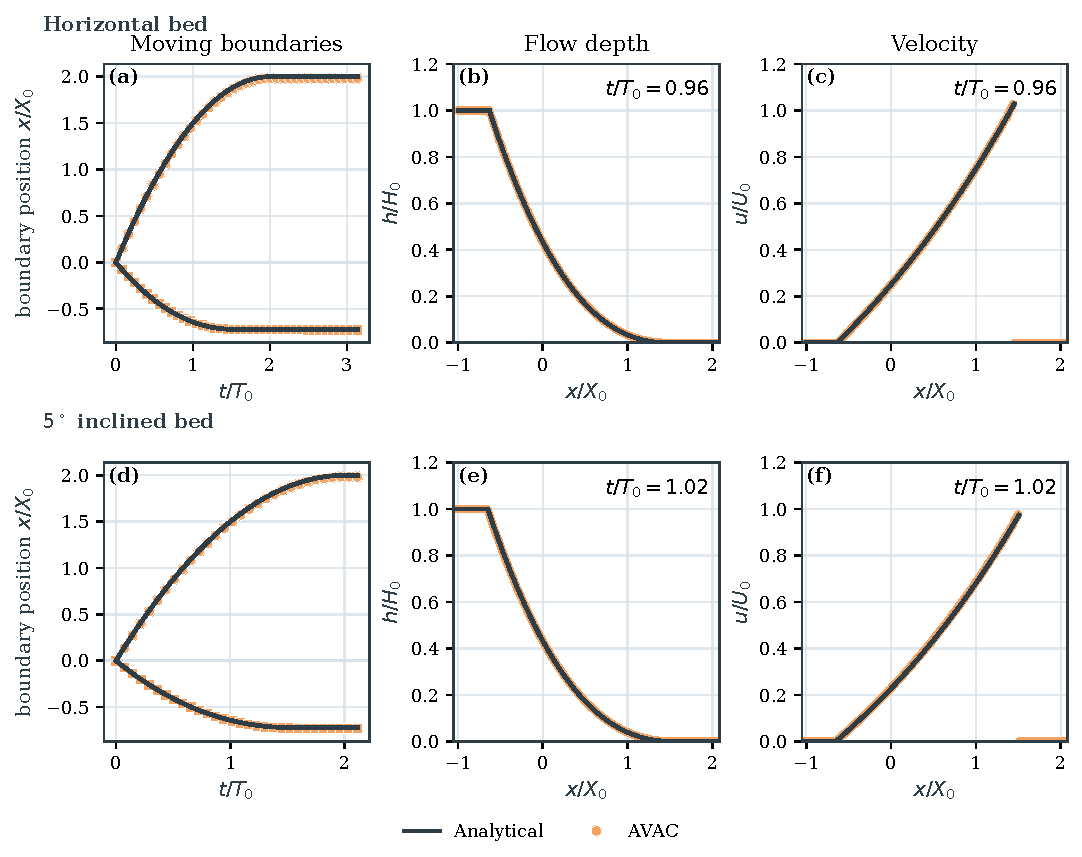
\includegraphics[width=\textwidth]{avac_coulomb_verification.pdf}
  \caption{AVAC verification against the Coulomb dam-break solution of
  \citet{Kerswell2005}.  The upper row shows the horizontal-bed case and the
  lower row the $5^\circ$ inclined-bed case.  Panels (a,d) compare the front
  (circles) and rear (squares) trajectories; panels (b,e) compare flow depth;
  and panels (c,f) compare downslope velocity at $t/T_0\simeq1$.  Dark lines
  denote the analytical solution and orange symbols denote AVAC centerline
  results.  AMR provides finest longitudinal spacings of
  \SI{2.5}{\milli\metre} and \SI{1.875}{\milli\metre} in the two rows,
  respectively. These are the supplied pre-1.0.0 verification fields
  (executable prefix \texttt{6e85bee646c3}), not a new release-wide AMR run.}
  \label{fig:avac-coulomb-verification}
\end{figure}

The two Coulomb tests are complementary.  The horizontal calculation shows
that AVAC propagates and arrests a finite granular mass without gravitational
driving along the bed, whereas the inclined calculation shows that the same
behavior is recovered after the driving and resisting accelerations are
combined.  Their common dimensionless solution therefore links the observed
agreement to the implementation of the AVAC source terms, rather than to a
case-specific parameter adjustment.

\subsubsection{Local curvature normal-load source}
\label{sec:avac-curvature-source-verification}

The curvature-dependent normal-load term was checked independently of the
finite-volume flux by compiling the same Fortran rheology module used by AVAC
and comparing its scalar frozen-coefficient update with closed solutions. A
material element with initial map speed \SI{8}{\metre\per\second} and
$\mu=0.30$ was evaluated for \SI{4}{\second} at the nadir of planar,
concave-circular, and convex-circular tracks. The circular radius was
\SI{40}{\metre}, giving $\kappa_v=\pm\SI{0.025}{\per\metre}$, and the
analytical equation was
\begin{equation}
  \frac{\mathrm dU_h}{\mathrm dt}
  =-\mu\left(g+\kappa_vU_h^2\right).
  \label{eq:avac-curvature-verification}
\end{equation}
The maximum absolute speed errors were below
\SI{3.2e-15}{\metre\per\second}. Repeating a \SI{2}{\second} update as
eight equal source substeps changed the result only at machine precision.

A zero-force test of the isolated \emph{scalar basal routine} leaves its input
map speed unchanged. It must not be interpreted as the behavior of the full
current source step, which first performs the separate terrain-tangent
transport. The production regression tests additionally exercise affine-bed
identity, tangent-speed preservation, the differential connection limit,
rotated two-dimensional geometry, physical boundaries and patch partitioning.
These checks test distinct operators rather than replace a resolved curved-DEM
trajectory or establish convergence of their split composition.

The circular-track values above verify the normal-load term for frozen local
geometry. Their convex state remains below the loss-of-contact threshold in
Eq.~\eqref{eq:avac-contact-speed}; that particular example does not exercise
the branch switch. Compiled source-stopping tests cover the corrected Voellmy
and cohesive-Voellmy zero-result handling, including near-dry states and
unchanged Coulomb/water controls. The released test sources retain these
separate scopes explicitly.



\subsection{WAVE verification}
\label{sec:wave-verification}

\subsubsection{Lake at rest}

The first WAVE test asks whether the lake initialization and the discretized
bathymetric source remain balanced before any avalanche source is applied.
The bed contains the smooth bump used by the Baines steady-flow test, while
the initial free surface is horizontal at \SI{2}{\metre}.  The
\SI{25}{\metre} by \SI{1}{\metre} domain is resolved with
\SI{0.05}{\metre} cells, the longitudinal boundaries are closed, and the
transverse boundaries are periodic.  The coupling file contains no active
source.  Consequently, the exact solution is a lake at rest for the complete
\SI{10}{\second} calculation.

The free-surface errors rose during the initial numerical adjustment and then
remained nearly constant (Fig.~\ref{fig:wave-analytical-verification}a).  The
largest $L_\infty$ and $L_2$ errors over all saved times were
\SI{6.37e-4}{\metre} and \SI{6.11e-5}{\metre}, respectively.  Thus the
topographic balance introduces a submillimetric disturbance, but no growing
wave.  This test is especially relevant to the coupled workflow: it places an
upper bound on the background signal against which an avalanche-generated
impulse must be distinguished.

\subsubsection{Thacker planar oscillation in a paraboloid}

The still-water calculation does not exercise shoreline motion.  We therefore
use the exact planar free-surface oscillation in a parabolic basin derived by
\citet{Thacker1981}, with reference values generated independently through
the SWASHES collection \citep{DelestreEtAl2013}.  A \SI{4}{\metre} square
basin is represented by a $100\times100$ grid, giving
\SI{0.04}{\metre} cells, and wall conditions are imposed on all four sides.
The calculation covers three complete oscillation periods, so that phase,
amplitude, and repeated wetting and drying all contribute to the final error.

Figure~\ref{fig:wave-analytical-verification}b compares the WAVE and
analytical centerline free surfaces over the parabolic topography after the
third period.  The WAVE centerline depth follows the analytical wet support
and profile closely;
the depth RMSE is \SI{1.27e-3}{\metre}, and the maximum absolute error is
\SI{2.84e-3}{\metre}.  Together with the lake-at-rest result, this shows that
WAVE both maintains a nominally stationary lake and transports a moving
shoreline through a genuinely two-dimensional basin without a systematic
phase shift visible at the reported resolution.

\begin{figure}[t]
  \centering
  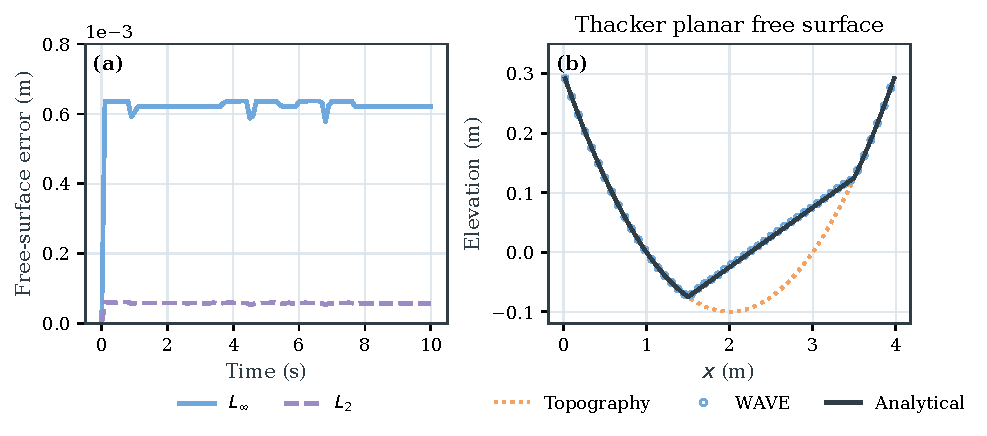
\includegraphics[width=\textwidth]{wave_analytical_verification.pdf}
  \caption{WAVE verification.  (a) $L_\infty$ and $L_2$ free-surface errors
  for the lake-at-rest test over a smooth bump.  (b) Centerline free surface
  after the third period of the planar Thacker oscillation in a parabolic
  basin.  Black is the analytical solution, blue open circles are WAVE, and
  orange dotted line is the topography.  Legends are placed outside the
  plotting regions.}
  \label{fig:wave-analytical-verification}
\end{figure}

The remaining analytical profiles and numerical diagnostics are collected in
Appendix~\ref{app:wave-verification}.  They broaden the evidence to steady
hydraulic transitions, shocks, friction, dry fronts, variable channel width,
AMR accuracy, and parallel reproducibility without interrupting the
stationary-to-moving-lake progression used here.




\subsection{Coupling verification}
\label{sec:coupling-verification}

The component tests above verify the two solvers separately, but not the
transfer between them.  We therefore prescribed a spatially uniform synthetic
AVAC state along a straight shoreline of length $L=\SI{0.8}{\metre}$.  Over
$T=\SI{1}{\second}$, its depth was $h_a=\SI{0.1}{\metre}$ and its velocity
was
\begin{equation}
  (u_a,v_a)=A(t)(0.02,0.01)\;\si{\metre\per\second}, \qquad
  A(t)=\sin(\pi t/T)\left(1+\frac{t}{4T}\right).
  \label{eq:coupling-verification-pulse}
\end{equation}
The pulse is zero at both ends and has closed-form volume and momentum
integrals.  It was written as native AVAC frames, sampled by the production
shoreline converter, serialized in the conservative source format, read by
the WAVE Fortran source module, and applied by the current WAVE executable.
Thus the test exercises the complete numerical transfer rather than only the
Python rate calculation.

For a uniform active shoreline, the expected transferred volume,
depth-integrated momentum, and physical water momentum are
\begin{align}
  V_w &= \beta L\int_0^T h_a u_n\,\mathrm{d}t, \\
  I_x &= \beta L\int_0^T h_a u_n u_a\,\mathrm{d}t, \qquad P_x=\rho_w I_x, \\
  I_y &= \beta L\int_0^T h_a u_n v_a\,\mathrm{d}t, \qquad P_y=\rho_w I_y,
  \label{eq:coupling-verification-ledger}
\end{align}
where $u_n$ is the velocity component directed into the lake and $\beta=1$
for this verification.  Equation~\eqref{eq:coupling-verification-pulse} gives
$V_w=\SI{1.14592e-3}{\metre\cubed}$,
$I_x=\SI{2.02827e-5}{\metre\tothe{4}\per\second}$, and
$I_y=\SI{1.01413e-5}{\metre\tothe{4}\per\second}$.  The WAVE domain was a
frictionless, periodic \SI{2}{\metre} by \SI{1}{\metre} basin with an
initial uniform depth of \SI{0.5}{\metre}.  Periodicity removes boundary
losses, so changes in the three globally integrated conserved variables can
be compared directly with the written source ledger.

The prescribed and serialized volume-rate histories are visually coincident
(Fig.~\ref{fig:coupling-verification}a).  WAVE was run on uniform
\SI{0.10}{\metre} and \SI{0.05}{\metre} grids and with two AMR levels from a
\SI{0.10}{\metre} base grid to a \SI{0.01}{\metre} finest grid.  Integration
of the non-overlapping native control volumes gave a maximum absolute relative
closure error of \num{5.61e-5} across volume and both momentum components
(Fig.~\ref{fig:coupling-verification}b).  The AMR run reached level 2 and
reduced the largest closure error to \num{2.95e-7}; the result therefore
confirms that the format-2 total rates remain conservative when the receiving
cell area changes.

\begin{figure}[t]
  \centering
  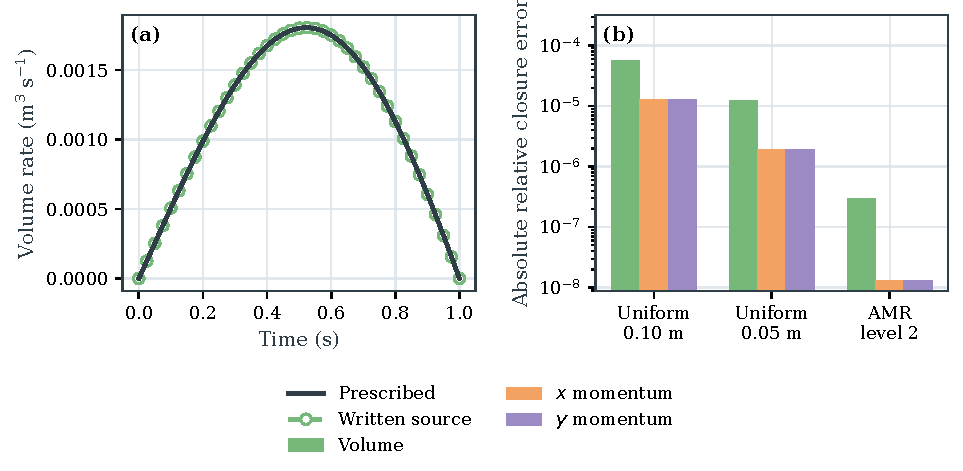
\includegraphics[width=\textwidth]{coupling_verification.pdf}
  \caption{Numerical verification of the AVAC-to-WAVE coupling.  (a)
  Prescribed and serialized volume-rate histories.  (b) Absolute relative
  closure errors for volume and both depth-momentum components on two uniform
  grids and a level-2 AMR grid.  The complete path includes native AVAC frames,
  the production converter and source file, the Fortran source update, and
  native WAVE control volumes.}
  \label{fig:coupling-verification}
\end{figure}

These tests verify numerical transfer and conservation, but they do not
validate the physical assumption that an entering avalanche can be replaced
by an equivalent one-way water source.  That question requires the planned
laboratory experiment in Sect.~\ref{sec:coupled-experiment}; the distinction
between numerical coupling verification and physical coupling validation is
maintained throughout this paper.






\newpage
\section{AVAC validation against observations}
\label{sec:avac-validation}

Before drafting this section, we must identify a comparable avalanche-model validation
paper with accessible release geometry, terrain, material parameters, and
observations of runout, front motion, velocity, or deposit. We should prefer an open
dataset and a case that permits either independently prescribed parameters or
calibration on one event followed by validation on another.  A single case
fitted and assessed with the same outputs must be described as calibration or
evaluation, not independent validation.








\newpage
\section{ISeeSnow avalanche-model intercomparison}
\label{sec:iseesnow}

\subsection{Protocol and common metrics}

The ISeeSnow v1.0 exercise provides common idealized and real topographies,
release areas, rheological parameters, and submitted peak fields from several
depth-integrated avalanche models \citep{WirbelEtAl2026}.  We ran AVAC on the
supplied \SI{5}{\metre} grid without retuning the prescribed physical
parameters. Numerical limiter and shallow-flow controls were assessed using
peer PFT comparisons, as distinguished below. The three calculations are the
idealized Voellmy case ($\mu=0.4$, $\xi=\SI{2000}{\metre\per\second\squared}$),
the real-topography Voellmy case ($\mu=0.2$ with the same $\xi$), and the
idealized Coulomb-only case ($\mu=0.4$ and no turbulent resistance).  In all
three cases, the prescribed terrain-normal release thickness is
\SI{1.5}{\metre}.

The two idealized cases share the same inclined plane, variable-width ravine,
release area, and flat foreland, while the real-terrain case uses a distinct
mountain catchment and release polygon (Fig.~\ref{fig:iseesnow-cases}).  Thus
the first and third calculations contrast Voellmy and Coulomb-only resistance
on a common geometry, using the model-specific numerical controls stated
below, whereas the first and
second retain Voellmy resistance while changing both terrain and the
prescribed Coulomb coefficient.

Because ISeeSnow prescribes release thickness normal to the terrain whereas
AVAC advances vertical map-cell depth, initialization applies the inverse
geometric conversion
\begin{equation}
  h_a(x,y,0)=\frac{h_n(x,y,0)}{\cos\phi(x,y)}.
  \label{eq:iseesnow-initial-depth}
\end{equation}
The prescribed normal release volume is therefore represented consistently
on sloping cells before the calculation begins.

\begin{figure}[t]
  \centering
  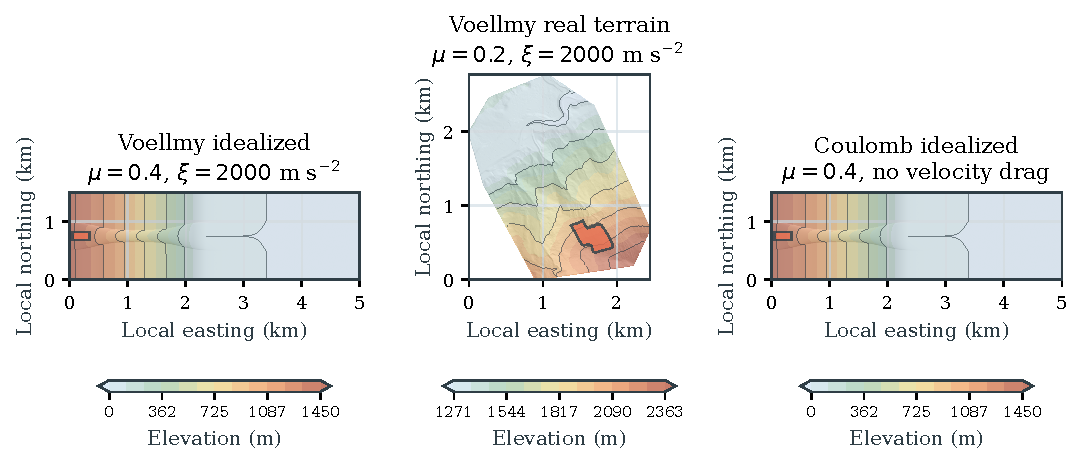
\includegraphics[width=\textwidth]{iseesnow_case_setup.pdf}
  \caption{The three AVAC ISeeSnow configurations, drawn from the supplied
  benchmark DEMs and release polygons.  (a) Idealized topography with Voellmy
  resistance, (b) real topography with Voellmy resistance, and (c) the same
  idealized topography with Coulomb resistance only.  Red polygons denote the
  common \SI{1.5}{\metre} terrain-normal release thickness.  The maps are an
  original rendering of the inputs used in \citet{WirbelEtAl2026}.}
  \label{fig:iseesnow-cases}
\end{figure}

AVAC stores vertical depth and horizontal map-coordinate momentum, whereas
ISeeSnow prescribes terrain-normal peak flow thickness (PFT). We therefore
convert vertical peak depth back to terrain-normal PFT cell by cell as
$\mathrm{PFT}_n=\mathrm{PFT}_h\cos\phi$. PFV is the physical terrain-tangent
magnitude consistent with Eq.~\eqref{eq:avac-geometry},
$[u_a^2+v_a^2+(u_a\partial_xB+v_a\partial_yB)^2]^{1/2}$, evaluated at every
solver step before taking the temporal maximum. The release state at $t=0$ is
included explicitly in the PFT maximum, and subsequent maxima are obtained
from the native peak-output calculation. PFV is zero for vertical depth at or
below \SI{0.05}{\metre}, uses the smooth diagnostic transition described in
Sect.~\ref{sec:avac-method} between \SI{0.05}{\metre} and
\SI{0.20}{\metre}, and is the exact terrain-tangent velocity at larger depth.
This follows the model-specific minimum-depth criteria documented by
ISeeSnow. The AVAC run configuration sets the shared GeoClaw speed limit to
$10^{99}$~\si{\metre\per\second}, so neither the evolving state nor the
reported PFV is clipped by a finite velocity ceiling.

Two peer populations serve different questions. The scalar overview uses the
published Table C1 core group: 11 idealized-Voellmy, 10 real-terrain, and
11 Coulomb submissions. It compares thalweg runout, maximum PFT and maximum
PFV. Runout is the furthest thalweg coordinate with normal PFT exceeding
\SI{0.5}{\metre}; it is not the area of a \SI{0.01}{\metre} support mask.
The off-scale Coulomb PFV of r.avaflow is retained in all scalar statistics
and annotated in the figure, not discarded.

Spatial PFT comparison, the primary numerical-selection criterion, instead
uses only rasters with exactly matching dimensions, cell size and sample
coordinates: 9, 8 and 8 peers for the three cases. No field is shifted or
resampled to improve agreement. Its dimensionless score is
\begin{equation}
 E_{\mathrm{PFT}} =
 \mathop{\mathrm{median}}_i
 \left[
 \frac{\mathrm{RMSE}(\mathrm{PFT}_{\mathrm{AVAC}},\mathrm{PFT}_i)}
 {\mathop{\mathrm{median}}_{j\ne i}
  \mathrm{RMSE}(\mathrm{PFT}_i,\mathrm{PFT}_j)}
 \right],
 \label{eq:iseesnow-pft-score}
\end{equation}
using full-grid errors and the recorded common nodata treatment. It is not
the unnormalized median RMSE in meters, nor an observational accuracy score.
The broader scalar population must not be confused with this spatially
aligned population.

All cases use a uniform \SI{5}{\metre} grid, second-order spatial updating,
a \SI{1200}{\second} horizon and \SI{10}{\second} saved-state intervals.
The two Voellmy cases use Van Leer and target CFL 0.50; Coulomb uses Minmod
and target CFL 0.25. The correction-flux depth controls are respectively
\SI{0.10}{\metre} and \SI{0.05}{\metre}; the solver dry tolerance is
\SI{1e-4}{\metre} and the rejection ceiling is CFL 1.0.

\subsection{Current fields and comparison with peers}

\begin{table}[htbp]
\centering
\caption{Accepted ISeeSnow results carried into version \modelversion.
The PFT score uses aligned spatial peers; the figure uses Table C1 scalars.}
\label{tab:iseesnow-current}
\small
\begin{tabular}{lrrrr}
\toprule
Case & Runout (km) & Peak PFT (m) & Peak PFV (m/s) & $E_{\mathrm{PFT}}$\\
\midrule
Idealized Voellmy & 2.31005 & 8.53216 & 39.6255 & 0.865517\\
Real-terrain Voellmy & 2.09712 & 21.03670 & 67.6648 & 0.907803\\
Idealized Coulomb & 3.15004 & 7.21983 & 110.9650 & 0.911514\\
\bottomrule
\end{tabular}
\end{table}

For idealized Voellmy, runout and peak PFT lie within the scalar peer
interquartile intervals, \SIrange{2.305}{2.335}{\kilo\metre} and
\SIrange{7.635}{9.285}{\metre}. Peak PFV is slightly above the upper quartile
of \SI{39.285}{\metre\per\second}, but below the peer maximum of
\SI{41.55}{\metre\per\second}. For real terrain, runout and peak PFT are
also within their interquartile intervals. PFV lies above the upper quartile
of \SI{52.465}{\metre\per\second}, within the full
\SIrange{40.87}{80.23}{\metre\per\second} range.

The Coulomb runout lies within the peer interquartile interval
\SIrange{3.13434}{3.22652}{\kilo\metre}. Peak PFT is slightly above its
upper quartile of \SI{7.125}{\metre}, while remaining within the
\SIrange{3.95}{9.97}{\metre} range. PFV is likewise just above its upper
quartile of \SI{110.7155}{\metre\per\second}. Thus the accepted Coulomb
runout is comparable with the central peer population, but the deposit crest
is not identical to a peer median. The peak normal thickness is
\SI{7.21983}{\metre}; its cell retains \SI{7.18942}{\metre} at the horizon
with zero momentum. The recorded direct-interface guard correction did not
alter this Coulomb trajectory relative to the preceding experimental V1
cohort: the complete saved native histories and final PFT/PFV fields match.
The crest is not attributed to that separately demonstrated guard defect.

The peer products are maxima over time, not observed final-deposit histories.
Different peer crests occur at different coordinates, so a pointwise median
can be lower than the median of their individual maxima. Neither a peer
envelope nor the scalar agreement in Table~\ref{tab:iseesnow-current}
identifies a unique physically correct deposit.

\begin{figure}[t]
  \centering
  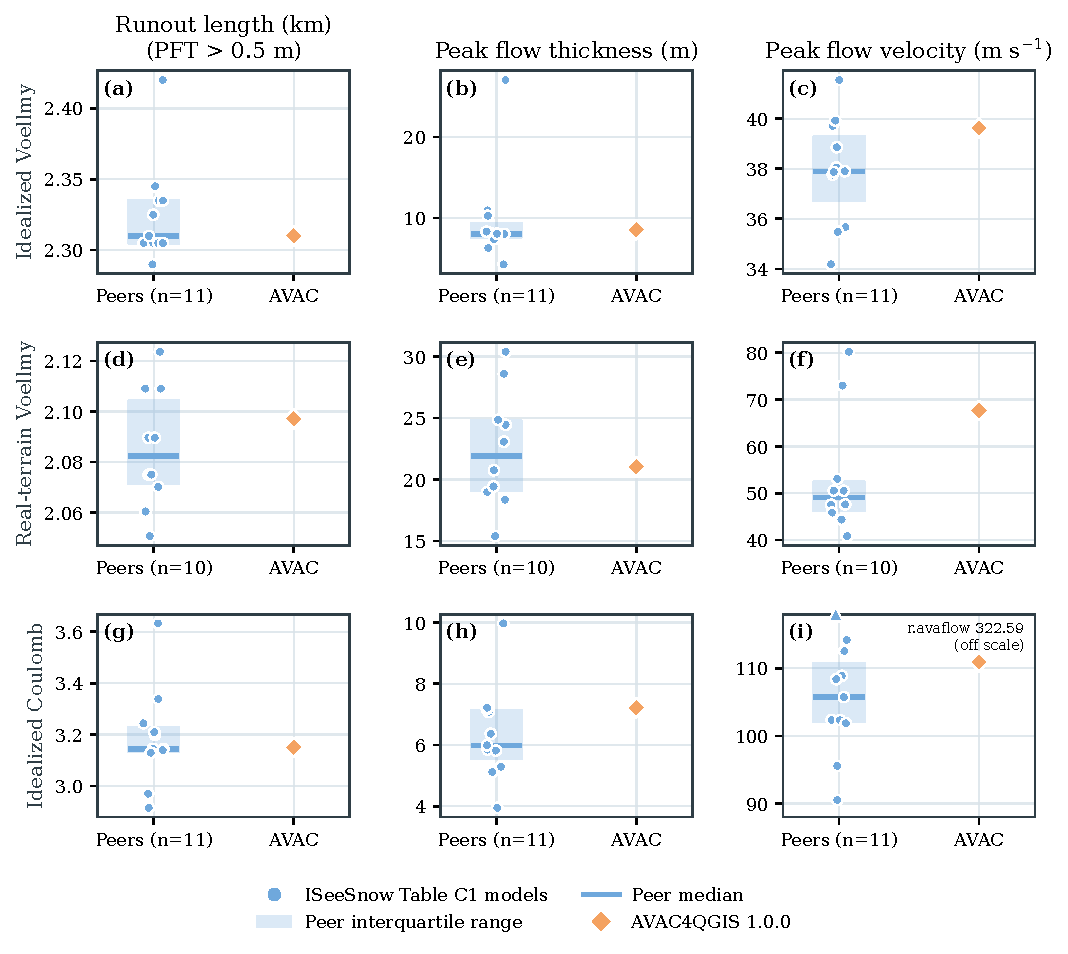
\includegraphics[width=\textwidth]{iseesnow_intercomparison_v1_0.pdf}
  \caption{Version \modelversion\ in the ISeeSnow Table C1 core-model
  ensemble. Rows show idealized Voellmy, real-terrain Voellmy and idealized
  Coulomb; columns show thalweg runout for PFT greater than
  \SI{0.5}{\metre}, peak PFT and peak PFV. Blue points, bands and lines are
  peer scalars, interquartile ranges and medians; orange diamonds are the
  accepted AVAC fields. All 11/10/11 peer values are retained. The off-scale
  Coulomb velocity is annotated and included in the statistics. This is a
  replot of authenticated completed-run metrics, not a newly executed
  validation experiment.}
  \label{fig:iseesnow-intercomparison}
\end{figure}

\subsection{Conservation, practical rest and remaining sensitivity}

The native relative volume changes $(V_f-V_0)/V_0$ are
\num{1.6463e-9}, \num{6.0960e-10} and \num{-6.4338e-10} for idealized
Voellmy, real-terrain Voellmy and Coulomb. Practical-rest confirmation occurs
at \SI{590}{\second}, \SI{520}{\second} and \SI{100}{\second}, respectively,
and remains satisfied at subsequent saved checks through the horizon.
This criterion requires less than 1\% of the release volume to be moving
faster than \SI{0.01}{\metre\per\second} in the resolved depth band above
\SI{0.05}{\metre}, for at least three saved times. It is not zero velocity in
every wet cell. Final resolved moving volumes are approximately
\SI{70.09}{\metre\cubed}, \SI{231.35}{\metre\cubed} and zero; motion below the
reporting-depth threshold is audited separately.

The correction that honors Voellmy's exact zero source result removed the
reproduced extremely large near-dry post-source states. Both full Voellmy
observation-only audits reproduced all 484 saved native artifacts and the
PFT/PFV fields; no invalid accepted post-source states were observed.
However, real terrain still has a raw all-step terrain-tangent maximum of
\SI{90.97}{\metre\per\second} in the \SIrange{0.05}{0.10}{\metre} depth band,
distinct from its filtered PFV of \SI{67.66}{\metre\per\second}. Neither saved
frames nor filtered peak fields bound every intermediate split state.

A same-source Voellmy target-CFL refinement from 0.50 to 0.25 reduced the
real-terrain thin-layer pulse and improved its normalized PFT score by about
1.52\%, but worsened the idealized PFT score by about 1.84\%. PFV and local
fields changed non-uniformly. Accordingly, the existing controls are retained;
two timestep levels do not establish a convergence rate or universal
stability. The improved PFT comparisons, the separate flat-control evidence
and these remaining sensitivities are reported together rather than treating
peer agreement as a substitute for numerical verification.






\newpage
\section{Coupled avalanche--impulse-wave validation experiment}
\label{sec:coupled-experiment}

Write after the planned laboratory experiment is completed.  Planned subsections:
\begin{enumerate}
  \item experimental geometry, material properties, release, water depth, and
        measurement uncertainty;
  \item AVAC motion and shoreline-arrival state;
  \item transferred volume and momentum ledger;
  \item WAVE gauge histories, amplitudes, wavelengths, and runup;
  \item sensitivity to $\beta$, grid spacing, shoreline representation, and
        AVAC output interval;
  \item discrepancies attributable to hydrostatic and one-way coupling
        assumptions.
\end{enumerate}
Reserve the terms ``coupling validation'' and ``validated coupled model'' until
the experiment and acceptance metrics justify them.

\newpage
\section{Discussion}
\label{sec:discussion}


Draft once all evidence is available.  Planned subsections:
\begin{enumerate}
  \item what component verification, AVAC validation, ISeeSnow, and the
        coupling experiment establish;
  \item physical meaning and limitations of the one-way shoreline transfer;
  \item hydrostatic/non-dispersive limitations of WAVE;
  \item grid, shoreline, and temporal-sampling sensitivities;
  \item accessibility and reproducibility through QGIS and managed runtimes;
  \item future two-way, multilayer, or dispersive developments.
\end{enumerate}
Scientific equivalence across Windows, macOS, and Linux should be assessed
with a common test case and declared numerical tolerances.

\newpage
\section{Conclusions}
\label{sec:conclusions}

Four short paragraphs: the model-system contribution; evidence for AVAC
and WAVE; evidence from ISeeSnow and the coupling experiment; and the final
scope-of-use statement.


\section{Code and data availability}
\label{sec:code-data}

The source code and plugins for Windows, macOS, and Linux are available as
version \modelversion\
at \url{https://github.com/cgotelli/AVAC-QGIS/releases/tag/v1.0.0}; the
integrated development branch is \texttt{main}. The editable manuscript,
bibliography, figures and replot script are stored under
\codepath{docs/article}. The release also provides the compiled methods PDF,
platform-specific plugin ZIP files, SHA-256 checksums, and runtime manifests.
The main source tree retains the validation drivers and tests;
third-party components and their supplied licenses are described in
\codepath{THIRD\_PARTY\_NOTICES.md}.

The ISeeSnow input geometry and peer submissions originate from the common
protocol of \citet{WirbelEtAl2026}. The updated scalar figure retains the
archived input-data hash, exact AVAC solver identity, Table C1 values and
portable replot data. It can be redrawn without a solver run. Selected final
PFT/PFV fields, controls, diagnostic reports and earlier worktree patches were
preserved in compact local evidence archives during release preparation;
bulk intermediate native histories were removed. Historical audit reports
remain records of the completed checks, but repeating their full byte-level
audits requires regenerating those histories. This repository deposit is not
claimed to have a DOI or to be a complete permanent archive of every
intermediate field. Planned observational and laboratory-validation data are
not represented as available results.

\newpage
\appendix

\section{Additional AVAC verification}
\label{app:avac-verification}

As an end-member test, AVAC was also configured with zero basal friction and
no avalanche rheology and compared with the exact finite-volume dam-break
solution of \citet{AnceyEtAl2008}.  A triangular prism of water with
$H_0=\SI{1}{\metre}$ was released on a frictionless $10^\circ$ planar bed;
its initial depth was
$h(x,0)=H_0(1-x/x_b)$ for $x_b\leq x\leq0$, where
$x_b=-H_0/\tan(10^\circ)$.  The calculation used the same three-level,
front-focused AMR procedure as the main AVAC tests on a domain extending from
$x=-\SI{10}{\metre}$ to $x=\SI{60}{\metre}$, progressing from a
\SI{40}{\milli\metre} background spacing to
\SI{2.5}{\milli\metre} near the head and tail.  This case is placed in the
appendix because it verifies the frictionless shallow-water limit shared with
GeoClaw, rather than avalanche-specific resistance.

A constant \SI{10}{\metre} vertical datum was retained in the planar-bed
input used for this benchmark. The present AVAC configuration sets GeoClaw's
reference sea level to $-10^4$~m, safely below the computational terrain, so
the translation is no longer required to keep newly refined dry cells dry.
It is nevertheless immaterial to the comparison because a uniform vertical
translation changes neither bed gradients, water depth, nor the analytical
solution.

The extended domain retained both moving boundaries throughout the complete
\SI{5}{\second} comparison.  Over that interval, the front and rear RMSEs
were \SI{0.06266}{\metre} and \SI{0.08056}{\metre}, respectively. The
maximum initial-depth discrepancy on
the uniform diagnostic grid was \SI{3.31}{\milli\metre}.  The initial depth
integral, \SI{2.83564}{\metre\squared} per meter of transverse width, differed
from the exact value by \SI{1.31e-7}{\metre\squared} and varied by
\SI{4.15e-4}{\metre\squared} over the full simulation, or
\SI{0.0146}{\percent}.  These errors include the interpolation from the
front-focused AMR hierarchy to the one-row diagnostic grid.

\FloatBarrier
\begin{figure}[htbp]
  \centering
  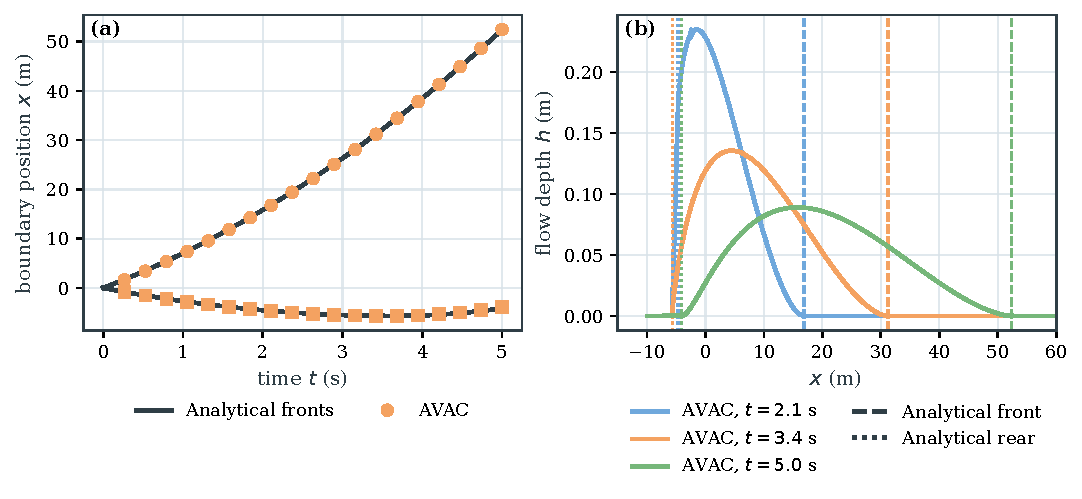
\includegraphics[width=\textwidth]{avac_wrr_water_limit.pdf}
  \caption{Frictionless AVAC water-limit verification against
  \citet{AnceyEtAl2008}.  (a) Analytical and numerical positions of the
  advancing front and rear boundary over the complete \SI{5}{\second}
  simulation.  (b) AVAC depth profiles at approximately \SI{2.1}{\second},
  \SI{3.4}{\second}, and \SI{5}{\second};
  dashed and dotted vertical lines mark the corresponding analytical front
  and rear positions.  The profiles are produced from saved centerline fields
  and are not solver inputs. This is the supplied historical checkpoint,
  not a newly executed version \modelversion\ benchmark.}
  \label{fig:avac-wrr-water-limit}
\end{figure}

The water-limit result completes a progression from frictionless acceleration
to Coulomb spreading on horizontal and inclined beds.  It confirms that the
underlying wet--dry and topographic terms retain their expected shallow-water
behavior before avalanche-specific resistance is activated.  Full numerical
controls and machine-readable error summaries accompany the executable
notebook, while the figure-generation notebook reads only those archived
products.

\newpage
\section{Additional WAVE verification}
\label{app:wave-verification}

The two main-paper tests were selected because they most directly represent a
stationary and an oscillating lake.  The remaining executable notebooks cover
steady hydraulic transitions, shocks, friction, a dry dam break, variable
channel width, and the accelerating sloping-bed solution.  Table~\ref{tab:wave-extra}
collects their principal depth errors using each benchmark's natural
one-dimensional or cross-section-mean diagnostic.  The SWASHES solutions were
generated from the pinned analytical implementation \citep{DelestreEtAl2013};
no numerical reference solver was used.

Figure~\ref{fig:wave-additional-benchmarks} shows selected saved numerical
profiles beside their analytical references.  The panels cover one-dimensional
hydraulic transitions, wet--dry propagation, and the full error histories for
the steady Baines bump and lake-at-rest configurations.

\begin{figure}[htbp]
  \centering
  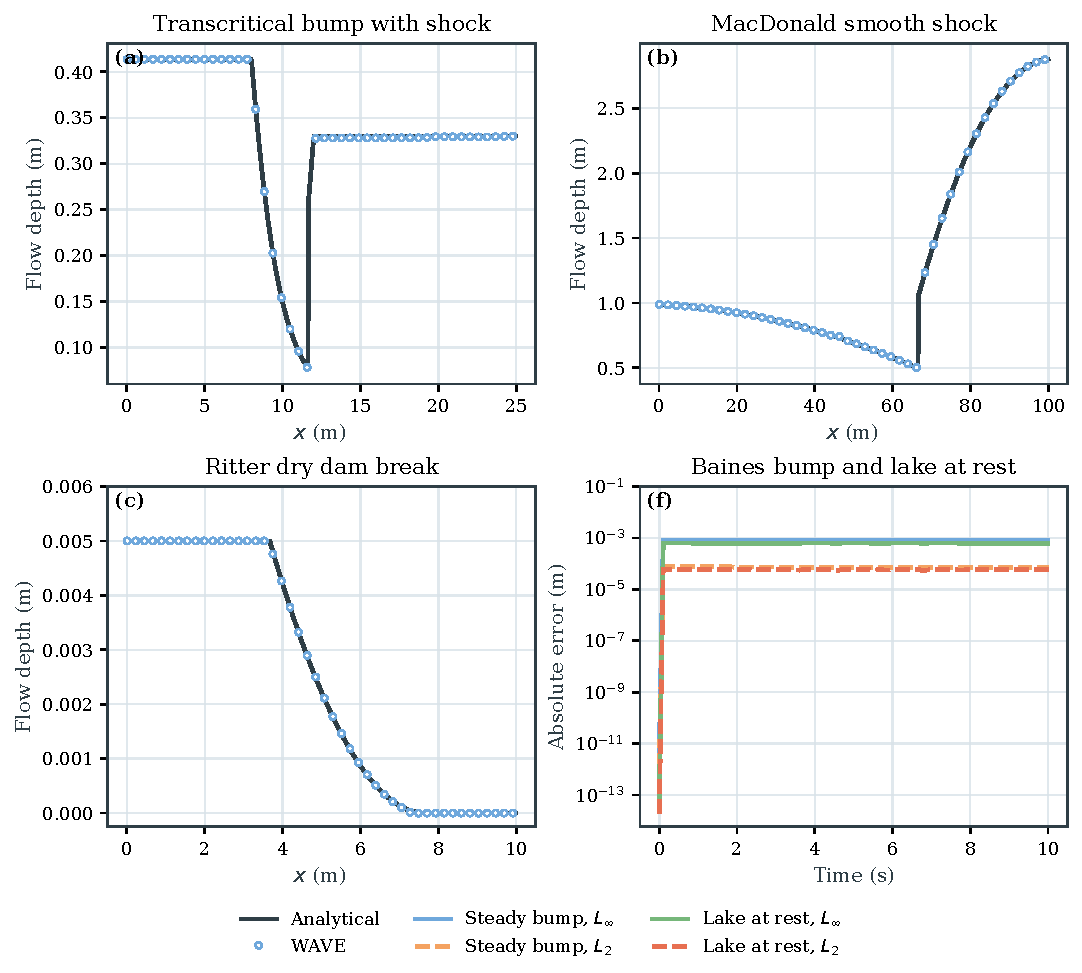
\includegraphics[width=\textwidth]{wave_additional_benchmarks.pdf}
  \caption{Additional WAVE analytical verification.  (a) Transcritical flow
  over a bump with a shock, (b) the MacDonald smooth-transition and shock
  solution, (c) the Ritter dry-bed dam break, and (f) the Baines steady-bump
  and lake-at-rest error histories.  Dark curves are
  analytical solutions, blue open circles are WAVE, and the pastel curves in
  (f) distinguish the two error norms and stationary tests.}
  \label{fig:wave-additional-benchmarks}
\end{figure}

\begin{table}[htbp]
  \centering
  \caption{Additional WAVE analytical-verification results.  ``Centerline''
  applies to the two-dimensional Thacker basin, and ``section mean'' to the
  variable-width pseudo-2D channels.}
  \label{tab:wave-extra}
  \small
  \begin{tabular}{lccc}
    \toprule
    Case and metric & $\Delta x$ (m) & RMSE (m) & Maximum error (m) \\
    \midrule
    Transcritical bump with shock, depth & 0.05 & \num{4.26e-3} & \num{9.15e-2} \\
    MacDonald smooth shock, depth & 0.20 & \num{7.72e-3} & \num{1.68e-1} \\
    Ritter dry dam break, depth & 0.02 & \num{1.07e-5} & \num{7.15e-5} \\
    Thacker paraboloid, centerline depth & 0.04 & \num{1.27e-3} & \num{2.84e-3} \\
    Pseudo-2D supercritical, section mean & 0.10 & \num{3.30e-2} & \num{1.05e-1} \\
    Pseudo-2D subcritical, section mean & 0.20 & \num{5.18e-2} & \num{8.36e-2} \\
    Baines steady bump, depth & 0.05 & \num{7.07e-5} & \num{7.80e-4} \\
    Lake at rest, free surface & 0.05 & \num{5.75e-5} & \num{6.21e-4} \\
    \bottomrule
  \end{tabular}
\end{table}

WAVE was also applied to the frictionless dry-bottom sloping-bed solution of
\citet{AnceyEtAl2008} with \SI{0.005}{\metre} cells.  Before its advancing
front reached the tutorial's open boundary, the front and rear RMSEs were
\SI{0.170}{\metre} and \SI{0.0274}{\metre}, respectively, while the initial
depth differed from the exact profile by at most
\SI{5.63e-13}{\metre}.  This independently exercises the water executable on
the same accelerating wet--dry problem used for AVAC in
Appendix~\ref{app:avac-verification}.

Finally, a flat-bed dry dam break compared a \SI{0.05}{\metre} uniform grid,
a \SI{0.005}{\metre} uniform reference, and level-2 AMR with the same finest
spacing.  AMR reduced the RMS depth difference from \SI{1.90e-3}{\metre} to
\SI{2.30e-4}{\metre}.  Repeating both the fine uniform and AMR calculations
with one and eight OpenMP threads produced byte-identical final native and
fixed-grid files.  Native non-overlapping AMR integration, rather than a
coarse visualization grid, gave a maximum relative mass change of
\num{4.68e-7} across the uniform and AMR configurations.

These last two diagnostics are summarized in
Fig.~\ref{fig:wave-numerical-diagnostics}.  The sloping-bed calculation tests
an accelerating wet--dry boundary before the open boundary is reached, while
the dam-break comparison shows the improvement obtained by concentrating the
fine spacing near the front.  Thread-count equality is reported separately
because coincident curves alone cannot establish bitwise reproducibility.

\begin{figure}[htbp]
  \centering
  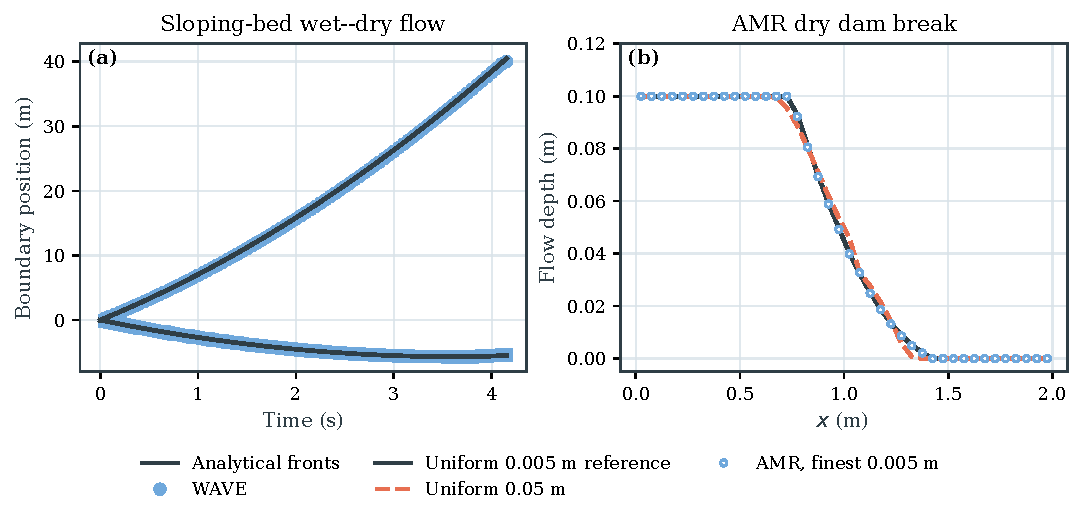
\includegraphics[width=\textwidth]{wave_numerical_diagnostics.pdf}
  \caption{WAVE wet--dry and numerical diagnostics.  (a) Front and rear
  trajectories for the frictionless sloping-bed solution before the advancing
  front reaches the open boundary.  (b) Final dry-dam-break depth on the
  uniform coarse grid and level-2 AMR grid, compared with the uniform fine
  reference.  The AMR markers use the same \SI{0.005}{\metre} finest spacing
  as the reference.}
  \label{fig:wave-numerical-diagnostics}
\end{figure}

\newpage
\section{Cross-platform reproducibility}
\label{app:platforms}

Version \modelversion\ provides plugin packages for Windows, macOS, and Linux.
Each package includes native solvers, Clawpack 5.14.0, required libraries,
and component licenses. Supported architectures, operating-system
requirements, checksums, and runtime inventories are documented with the
release.

The Windows AMD64 build supports QGIS 3.40 or newer. Its earlier isolated
functional test used QGIS 3.40.11-Bratislava: AVAC and WAVE runtimes
installed automatically and an AVAC
run completed. That offscreen QGIS process subsequently crashed at shutdown,
so its functional pass is not a clean-exit certification. The version
\modelversion\ packaging and isolated-runtime installation checks are separate
from that earlier GUI run.

For the Windows package, the AVAC and WAVE executable SHA-256 values are,
respectively,
\begin{quote}\small
\path{55a8c4baf0cc74d9a8ca4c582f361eb85ab01817b0d16b63e1c824611144f2e3}\\
\path{05bbcc28e71554cf13d1cc76c05329af1eb42a2966a8ec4738ef0310b9cbc555}.
\end{quote}
These executables are unchanged from the accepted Windows 0.6.1 package;
runtime-version metadata and plugin release descriptors were updated to
1.0.0.

The macOS package targets Apple Silicon and macOS 14.0 or newer. A clean QGIS
3.44.12-Solothurn profile test installed both runtimes, prepared an AVAC case,
and completed the simulation with the expected time-dependent and peak
outputs. This test was performed on the available Apple Silicon system,
not on a separate macOS 14 installation.

Linux is also supported by an installable package. Platform availability and
installation tests do not establish numerical equivalence across operating
systems. A common scientific test suite with stated tolerances is needed for
that comparison.

\newpage
\bibliographystyle{plainnat}
\bibliography{references}


\end{document}
